% PrepLang as an Original Software Publication (OSP) for the Software Track of Science of Computer
% Programming, on Elsevier's OSP template (scico-osp-template.tex): code metadata table, motivation,
% software description, illustrative example, impact, conclusions. Suggested length 3-6 pages of
% running text. The research article is preplang-scp.tex.
% Build from this folder: py -3 ../eval/paper_numbers.py, pdflatex preplang-osp.tex,
% py -3 osp_references.py, then pdflatex preplang-osp.tex twice.
\documentclass[preprint,12pt,a4paper]{elsarticle}  % the OSP template's settings, unchanged

\usepackage{lmodern}
\usepackage[T1]{fontenc}
\usepackage{microtype}
\DisableLigatures[-]{encoding=T1, family=tt*}  % --approx, not an en dash
\usepackage{amssymb}
\usepackage{xcolor}
\usepackage{listings}
\usepackage{array}
\usepackage{adjustbox}
\usepackage{booktabs}
\usepackage{enumitem}
\setlist{itemsep=2pt, topsep=4pt, parsep=0pt}  % compact lists
\usepackage{xspace}
\usepackage{tikz}
\usetikzlibrary{arrows.meta}
\usepackage[hidelinks]{hyperref}
\setlength{\emergencystretch}{3em}

% Every measured number comes from eval/results/ through eval/paper_numbers.py.
% Generated by eval/paper_numbers.py from eval/results/. Do not edit.
\newcommand{\RqOneMsMin}{22}
\newcommand{\RqOneMsMax}{39}
\newcommand{\RqOneMsMed}{29}
\newcommand{\TabOpt}{1.49}
\newcommand{\TabOz}{1.81}
\newcommand{\TabBase}{1.82}
\newcommand{\TabSpeedup}{1.21}
\newcommand{\TabStart}{1.02}
\newcommand{\TabProcOpt}{0.47}
\newcommand{\TabProcOz}{0.79}
\newcommand{\TabCut}{40}
\newcommand{\ImgPl}{3.52}
\newcommand{\ImgPlMem}{10}
\newcommand{\ImgBase}{4.01}
\newcommand{\ImgBaseMem}{922}
\newcommand{\ImgHw}{3.54}
\newcommand{\ImgHwMem}{12}
\newcommand{\FusExact}{5.56}
\newcommand{\FusApprox}{5.26}
\newcommand{\FusSave}{5}
\newcommand{\FusPsnr}{57.0}
\newcommand{\FusPsnrMin}{51.8}
\newcommand{\CsvTenK}{0.01}
\newcommand{\CsvTenKRead}{0.06}
\newcommand{\CsvHundredK}{0.03}
\newcommand{\CsvHundredKRead}{0.08}
\newcommand{\CsvMillion}{0.13}
\newcommand{\CsvMillionRead}{0.62}
\newcommand{\ImgHundred}{0.02}
\newcommand{\ImgHundredRead}{0.14}
\newcommand{\ImgThousand}{0.08}
\newcommand{\ImgThousandRead}{1.48}
\newcommand{\ImgThreeK}{0.33}
\newcommand{\ImgThreeKRead}{5.73}
\newcommand{\CsvRatio}{0.2}
\newcommand{\CsvSpeedup}{4.7}
\newcommand{\CsvArrowRead}{0.11}
\newcommand{\CsvArrow}{0.8}
\newcommand{\HdrRatio}{17}
\newcommand{\PqOne}{0.015}
\newcommand{\PqOneRead}{0.66}
\newcommand{\PqOneSize}{22}
\newcommand{\PqFour}{0.016}
\newcommand{\PqFourRead}{0.19}
\newcommand{\PqFourSize}{87}
\newcommand{\PqSixteen}{0.018}
\newcommand{\PqSixteenRead}{0.84}
\newcommand{\PqSixteenSize}{346}
\newcommand{\ScTabOkPl}{0.02}
\newcommand{\ScTabOkScript}{4.51}
\newcommand{\ScTabOkRun}{4.74}
\newcommand{\ScTabNamePl}{0.02}
\newcommand{\ScTabNameScript}{2.81}
\newcommand{\ScTabContractPl}{0.02}
\newcommand{\ScTabContractScript}{1.79}
\newcommand{\ScImgOkPl}{0.33}
\newcommand{\ScImgOkScript}{8.53}
\newcommand{\ScImgOkRun}{10.51}
\newcommand{\ScImgBrokenPl}{0.26}
\newcommand{\ScImgBrokenScript}{9.15}
\newcommand{\ScImgFloatPl}{0.26}
\newcommand{\ScImgFloatScript}{8.54}
\newcommand{\RbTotal}{44}
\newcommand{\RbEarly}{18}
\newcommand{\RbEarlyPct}{41}
\newcommand{\RbCompile}{12}
\newcommand{\RbContract}{6}
\newcommand{\RbDesign}{3}
\newcommand{\RbNone}{23}
\newcommand{\RbBefore}{15}
\newcommand{\RbBeforePct}{34}
\newcommand{\RbCases}{21}
\newcommand{\RbPass}{21}
\newcommand{\RbFormat}{6}
\newcommand{\RbOperation}{5}
\newcommand{\RbDates}{4}
\newcommand{\RbLabels}{3}
\newcommand{\RbProduced}{2}
\newcommand{\RbContractMissing}{2}
\newcommand{\RbModel}{1}
\newcommand{\CertBatches}{244}
\newcommand{\CertDeopted}{35}
\newcommand{\CertRescued}{35}
\newcommand{\CertFpCorrect}{115}
\newcommand{\CertFpNeedless}{129}
\newcommand{\CertFpUnsound}{0}
\newcommand{\CertFpCorrectPct}{47}
\newcommand{\CertFpNeedlessPct}{53}
\newcommand{\CertFactsCorrect}{122}
\newcommand{\CertFactsNeedless}{81}
\newcommand{\CertFactsUnsound}{41}
\newcommand{\CertFactsCorrectPct}{50}
\newcommand{\CertFactsNeedlessPct}{33}
\newcommand{\CertPanderaAllCorrect}{121}
\newcommand{\CertPanderaAllNeedless}{82}
\newcommand{\CertPanderaAllUnsound}{41}
\newcommand{\CertPanderaAllCorrectPct}{50}
\newcommand{\CertPanderaAllNeedlessPct}{34}
\newcommand{\CertPanderaReadCorrect}{124}
\newcommand{\CertPanderaReadNeedless}{79}
\newcommand{\CertPanderaReadUnsound}{41}
\newcommand{\CertPanderaReadCorrectPct}{51}
\newcommand{\CertPanderaReadNeedlessPct}{32}
\newcommand{\CertGxAllCorrect}{138}
\newcommand{\CertGxAllNeedless}{106}
\newcommand{\CertGxAllUnsound}{0}
\newcommand{\CertGxAllCorrectPct}{57}
\newcommand{\CertGxAllNeedlessPct}{43}
\newcommand{\CertGxReadCorrect}{140}
\newcommand{\CertGxReadNeedless}{104}
\newcommand{\CertGxReadUnsound}{0}
\newcommand{\CertGxReadCorrectPct}{57}
\newcommand{\CertGxReadNeedlessPct}{43}
\newcommand{\CertTfdvAllCorrect}{147}
\newcommand{\CertTfdvAllNeedless}{31}
\newcommand{\CertTfdvAllUnsound}{66}
\newcommand{\CertTfdvAllCorrectPct}{60}
\newcommand{\CertTfdvAllNeedlessPct}{13}
\newcommand{\CertTfdvReadCorrect}{150}
\newcommand{\CertTfdvReadNeedless}{28}
\newcommand{\CertTfdvReadUnsound}{66}
\newcommand{\CertTfdvReadCorrectPct}{61}
\newcommand{\CertTfdvReadNeedlessPct}{11}
\newcommand{\CertFullCorrect}{244}
\newcommand{\CertFullNeedless}{0}
\newcommand{\CertFullUnsound}{0}
\newcommand{\CertFullCorrectPct}{100}
\newcommand{\CertFullNeedlessPct}{0}
\newcommand{\CertDeoptCorrect}{244}
\newcommand{\CertDeoptNeedless}{0}
\newcommand{\CertDeoptUnsound}{0}
\newcommand{\CertDeoptCorrectPct}{100}
\newcommand{\CertDeoptNeedlessPct}{0}
\newcommand{\RealRuns}{238}
\newcommand{\RealDeopted}{9}
\newcommand{\RealRescued}{9}
\newcommand{\RealFreshFails}{17}
\newcommand{\RealTypeRefusals}{24}
\newcommand{\RealFpCorrect}{17}
\newcommand{\RealFpNeedless}{221}
\newcommand{\RealFpUnsound}{0}
\newcommand{\RealFpCorrectPct}{7}
\newcommand{\RealFpNeedlessPct}{93}
\newcommand{\RealFactsCorrect}{19}
\newcommand{\RealFactsNeedless}{219}
\newcommand{\RealFactsUnsound}{0}
\newcommand{\RealFactsCorrectPct}{8}
\newcommand{\RealFactsNeedlessPct}{92}
\newcommand{\RealPanderaAllCorrect}{19}
\newcommand{\RealPanderaAllNeedless}{219}
\newcommand{\RealPanderaAllUnsound}{0}
\newcommand{\RealPanderaAllCorrectPct}{8}
\newcommand{\RealPanderaAllNeedlessPct}{92}
\newcommand{\RealPanderaReadCorrect}{19}
\newcommand{\RealPanderaReadNeedless}{219}
\newcommand{\RealPanderaReadUnsound}{0}
\newcommand{\RealPanderaReadCorrectPct}{8}
\newcommand{\RealPanderaReadNeedlessPct}{92}
\newcommand{\RealGxAllCorrect}{17}
\newcommand{\RealGxAllNeedless}{221}
\newcommand{\RealGxAllUnsound}{0}
\newcommand{\RealGxAllCorrectPct}{7}
\newcommand{\RealGxAllNeedlessPct}{93}
\newcommand{\RealGxReadCorrect}{17}
\newcommand{\RealGxReadNeedless}{221}
\newcommand{\RealGxReadUnsound}{0}
\newcommand{\RealGxReadCorrectPct}{7}
\newcommand{\RealGxReadNeedlessPct}{93}
\newcommand{\RealTfdvAllCorrect}{51}
\newcommand{\RealTfdvAllNeedless}{163}
\newcommand{\RealTfdvAllUnsound}{24}
\newcommand{\RealTfdvAllCorrectPct}{21}
\newcommand{\RealTfdvAllNeedlessPct}{68}
\newcommand{\RealTfdvReadCorrect}{138}
\newcommand{\RealTfdvReadNeedless}{73}
\newcommand{\RealTfdvReadUnsound}{27}
\newcommand{\RealTfdvReadCorrectPct}{58}
\newcommand{\RealTfdvReadNeedlessPct}{31}
\newcommand{\RealFullCorrect}{215}
\newcommand{\RealFullNeedless}{23}
\newcommand{\RealFullUnsound}{0}
\newcommand{\RealFullCorrectPct}{90}
\newcommand{\RealFullNeedlessPct}{10}
\newcommand{\RealDeoptCorrect}{221}
\newcommand{\RealDeoptNeedless}{17}
\newcommand{\RealDeoptUnsound}{0}
\newcommand{\RealDeoptCorrectPct}{93}
\newcommand{\RealDeoptNeedlessPct}{7}
\newcommand{\RealValidatorStopMin}{92}
\newcommand{\RealValidatorStopMax}{93}
\newcommand{\RealValidatorWrongMax}{27}
\newcommand{\CorpusAll}{372}
\newcommand{\CorpusTest}{272}
\newcommand{\CorpusLifted}{130}
\newcommand{\CorpusCompiled}{124}
\newcommand{\CorpusStatements}{189}
\newcommand{\CorpusChanges}{328}
\newcommand{\CorpusComplete}{30}
\newcommand{\CorpusRuns}{1364}
\newcommand{\CorpusAdmit}{1357}
\newcommand{\CorpusAdmitPct}{99}
\newcommand{\CorpusSame}{1357}
\newcommand{\CorpusUnsound}{0}
\newcommand{\CorpusStopped}{0}
\newcommand{\CorpusStoppedRuns}{0}
\newcommand{\CorpusRefusedCrash}{7}
\newcommand{\CorpusRefusedRuns}{0}
\newcommand{\CorpusDeopted}{10}
\newcommand{\CorpusFullAdmit}{1347}
\newcommand{\CorpusFullSame}{1347}
\newcommand{\CorpusFullUnsound}{0}
\newcommand{\CorpusFullRefusedRuns}{10}
\newcommand{\HousesAll}{461}
\newcommand{\HousesTest}{461}
\newcommand{\HousesLifted}{168}
\newcommand{\HousesCompiled}{168}
\newcommand{\HousesStatements}{208}
\newcommand{\HousesChanges}{377}
\newcommand{\HousesComplete}{48}
\newcommand{\HousesRuns}{1848}
\newcommand{\HousesAdmit}{1841}
\newcommand{\HousesAdmitPct}{100}
\newcommand{\HousesSame}{1841}
\newcommand{\HousesUnsound}{0}
\newcommand{\HousesStopped}{0}
\newcommand{\HousesStoppedRuns}{0}
\newcommand{\HousesRefusedCrash}{7}
\newcommand{\HousesRefusedRuns}{0}
\newcommand{\HousesDeopted}{3}
\newcommand{\HousesFullAdmit}{1838}
\newcommand{\HousesFullSame}{1838}
\newcommand{\HousesFullUnsound}{0}
\newcommand{\HousesFullRefusedRuns}{3}
\newcommand{\CorpusBothScripts}{733}
\newcommand{\CorpusBothRuns}{3212}
\newcommand{\CorpusBothSame}{3198}
\newcommand{\CorpusBothLifted}{292}
\newcommand{\CorpusDerAll}{372}
\newcommand{\CorpusDerTest}{272}
\newcommand{\CorpusDerLifted}{130}
\newcommand{\CorpusDerCompiled}{124}
\newcommand{\CorpusDerStatements}{199}
\newcommand{\CorpusDerChanges}{337}
\newcommand{\CorpusDerComplete}{31}
\newcommand{\CorpusDerRuns}{1364}
\newcommand{\CorpusDerAdmit}{1357}
\newcommand{\CorpusDerAdmitPct}{99}
\newcommand{\CorpusDerSame}{1357}
\newcommand{\CorpusDerUnsound}{0}
\newcommand{\CorpusDerStopped}{0}
\newcommand{\CorpusDerStoppedRuns}{0}
\newcommand{\CorpusDerRefusedCrash}{7}
\newcommand{\CorpusDerRefusedRuns}{0}
\newcommand{\CorpusDerDeopted}{10}
\newcommand{\CorpusDerFullAdmit}{1347}
\newcommand{\CorpusDerFullSame}{1347}
\newcommand{\CorpusDerFullUnsound}{0}
\newcommand{\CorpusDerFullRefusedRuns}{10}
\newcommand{\HousesDerAll}{461}
\newcommand{\HousesDerTest}{461}
\newcommand{\HousesDerLifted}{168}
\newcommand{\HousesDerCompiled}{168}
\newcommand{\HousesDerStatements}{263}
\newcommand{\HousesDerChanges}{431}
\newcommand{\HousesDerComplete}{48}
\newcommand{\HousesDerRuns}{1848}
\newcommand{\HousesDerAdmit}{1841}
\newcommand{\HousesDerAdmitPct}{100}
\newcommand{\HousesDerSame}{1841}
\newcommand{\HousesDerUnsound}{0}
\newcommand{\HousesDerStopped}{0}
\newcommand{\HousesDerStoppedRuns}{0}
\newcommand{\HousesDerRefusedCrash}{7}
\newcommand{\HousesDerRefusedRuns}{0}
\newcommand{\HousesDerDeopted}{3}
\newcommand{\HousesDerFullAdmit}{1838}
\newcommand{\HousesDerFullSame}{1838}
\newcommand{\HousesDerFullUnsound}{0}
\newcommand{\HousesDerFullRefusedRuns}{3}
\newcommand{\CorpusBothDerRuns}{3212}
\newcommand{\CorpusBothDerSame}{3198}
\newcommand{\CorpusBothDerUnsound}{0}
\newcommand{\CorpusBothDerStatements}{462}
\newcommand{\CorpusBothDerCompiled}{292}
\newcommand{\CorpusBothDerDeopted}{13}
\newcommand{\CorpusBothStatements}{397}
\newcommand{\DriftTrafficAll}{241}
\newcommand{\DriftTrafficLifted}{42}
\newcommand{\DriftTrafficCompiled}{41}
\newcommand{\DriftTrafficCompileErrors}{1}
\newcommand{\DriftTrafficStatements}{104}
\newcommand{\DriftTrafficDerive}{51}
\newcommand{\DriftTrafficWithRemovals}{3}
\newcommand{\DriftTrafficDatesAdmitted}{35}
\newcommand{\DriftTrafficParseDate}{36}
\newcommand{\DriftTrafficRuns}{2542}
\newcommand{\DriftTrafficSame}{2542}
\newcommand{\DriftTrafficWrong}{0}
\newcommand{\DriftTrafficStops}{0}
\newcommand{\DriftTrafficNeedless}{0}
\newcommand{\DriftTrafficDeopted}{6}
\newcommand{\DriftTrafficFullSame}{2536}
\newcommand{\DriftTrafficFullWrong}{0}
\newcommand{\DriftTrafficFullNeedless}{6}
\newcommand{\DriftBikesAll}{254}
\newcommand{\DriftBikesLifted}{19}
\newcommand{\DriftBikesCompiled}{19}
\newcommand{\DriftBikesCompileErrors}{0}
\newcommand{\DriftBikesStatements}{38}
\newcommand{\DriftBikesDerive}{22}
\newcommand{\DriftBikesWithRemovals}{0}
\newcommand{\DriftBikesDatesAdmitted}{9}
\newcommand{\DriftBikesParseDate}{9}
\newcommand{\DriftBikesRuns}{437}
\newcommand{\DriftBikesSame}{437}
\newcommand{\DriftBikesWrong}{0}
\newcommand{\DriftBikesStops}{0}
\newcommand{\DriftBikesNeedless}{0}
\newcommand{\DriftBikesDeopted}{0}
\newcommand{\DriftBikesFullSame}{437}
\newcommand{\DriftBikesFullWrong}{0}
\newcommand{\DriftBikesFullNeedless}{0}
\newcommand{\DriftHoursAll}{450}
\newcommand{\DriftHoursLifted}{12}
\newcommand{\DriftHoursCompiled}{12}
\newcommand{\DriftHoursCompileErrors}{0}
\newcommand{\DriftHoursStatements}{21}
\newcommand{\DriftHoursDerive}{7}
\newcommand{\DriftHoursWithRemovals}{1}
\newcommand{\DriftHoursDatesAdmitted}{7}
\newcommand{\DriftHoursParseDate}{7}
\newcommand{\DriftHoursRuns}{276}
\newcommand{\DriftHoursSame}{276}
\newcommand{\DriftHoursWrong}{0}
\newcommand{\DriftHoursStops}{0}
\newcommand{\DriftHoursNeedless}{0}
\newcommand{\DriftHoursDeopted}{0}
\newcommand{\DriftHoursFullSame}{276}
\newcommand{\DriftHoursFullWrong}{0}
\newcommand{\DriftHoursFullNeedless}{0}
\newcommand{\DriftAll}{945}
\newcommand{\DriftLifted}{73}
\newcommand{\DriftCompiled}{72}
\newcommand{\DriftCompileErrors}{1}
\newcommand{\DriftStatements}{163}
\newcommand{\DriftDerive}{80}
\newcommand{\DriftWithRemovals}{4}
\newcommand{\DriftDatesAdmitted}{51}
\newcommand{\DriftParseDate}{52}
\newcommand{\DriftRuns}{3255}
\newcommand{\DriftSame}{3255}
\newcommand{\DriftWrong}{0}
\newcommand{\DriftStops}{0}
\newcommand{\DriftNeedless}{0}
\newcommand{\DriftDeopted}{6}
\newcommand{\DriftFullSame}{3249}
\newcommand{\DriftFullWrong}{0}
\newcommand{\DriftFullNeedless}{6}
\newcommand{\DriftHeldAll}{704}
\newcommand{\DriftHeldLifted}{31}
\newcommand{\DriftHeldCompiled}{31}
\newcommand{\DriftHeldCompileErrors}{0}
\newcommand{\DriftHeldStatements}{59}
\newcommand{\DriftHeldDerive}{29}
\newcommand{\DriftHeldWithRemovals}{1}
\newcommand{\DriftHeldDatesAdmitted}{16}
\newcommand{\DriftHeldParseDate}{16}
\newcommand{\DriftHeldRuns}{713}
\newcommand{\DriftHeldSame}{713}
\newcommand{\DriftHeldWrong}{0}
\newcommand{\DriftHeldStops}{0}
\newcommand{\DriftHeldNeedless}{0}
\newcommand{\DriftHeldDeopted}{0}
\newcommand{\DriftHeldFullSame}{713}
\newcommand{\DriftHeldFullWrong}{0}
\newcommand{\DriftHeldFullNeedless}{0}
\newcommand{\ComposeFacts}{38}
\newcommand{\ComposeGuaranteed}{33}
\newcommand{\ComposeStageOneStops}{9}
\newcommand{\ComposeLikeFresh}{196}
\newcommand{\ComposeMonths}{196}
\newcommand{\ComposeBroken}{0}
\newcommand{\OhMonths}{92}
\newcommand{\OhTrusted}{0.88}
\newcommand{\OhFull}{0.88}
\newcommand{\OhDeopt}{0.88}
\newcommand{\OhPct}{$-1$}
\newcommand{\OhPctLow}{$-3$}
\newcommand{\OhPctHigh}{$+1$}
\newcommand{\OhCompile}{0.03}
\newcommand{\OhCompileMs}{28}
\newcommand{\OhFresh}{0.94}
\newcommand{\ImgBatches}{30}
\newcommand{\ImgBFpCorrect}{5}
\newcommand{\ImgBFpNeedless}{25}
\newcommand{\ImgBFpUnsound}{0}
\newcommand{\ImgBFpCorrectPct}{17}
\newcommand{\ImgBFpNeedlessPct}{83}
\newcommand{\ImgBFullCorrect}{10}
\newcommand{\ImgBFullNeedless}{20}
\newcommand{\ImgBFullUnsound}{0}
\newcommand{\ImgBFullCorrectPct}{33}
\newcommand{\ImgBFullNeedlessPct}{67}
\newcommand{\ImgBDeoptCorrect}{25}
\newcommand{\ImgBDeoptNeedless}{5}
\newcommand{\ImgBDeoptUnsound}{0}
\newcommand{\ImgBDeoptCorrectPct}{83}
\newcommand{\ImgBDeoptNeedlessPct}{17}
\newcommand{\ImgBTrustedUnsound}{15}
\newcommand{\ImgBDeopted}{15}
\newcommand{\CcPrograms}{11}
\newcommand{\CcAnalysesMin}{14}
\newcommand{\CcAnalysesMax}{207}
\newcommand{\CcFullAnalysesMax}{122}
\newcommand{\CcMsMin}{21}
\newcommand{\CcMsMax}{35}
\newcommand{\CcRatioMax}{2.3}
\newcommand{\CsPrograms}{8}
\newcommand{\CsFullMin}{6}
\newcommand{\CsFullMax}{17}
\newcommand{\CsItems}{23}
\newcommand{\CsItemMin}{1}
\newcommand{\CsItemMax}{2}
\newcommand{\CsAdmissionTypesOnly}{yes}
\newcommand{\CsTrafficCols}{6}
\newcommand{\CsTrafficFileCols}{9}
\newcommand{\CsBikesCols}{7}
\newcommand{\CsBikesFileCols}{16}
\newcommand{\CsTaxiCols}{9}
\newcommand{\CsTaxiFileCols}{20}
\newcommand{\PrivCompilations}{4,879}
\newcommand{\PrivRuns}{64,179}
\newcommand{\PrivUnsound}{0}
\newcommand{\PrivNeedless}{1168}
\newcommand{\PrivRandom}{398}
\newcommand{\PrivRandomRuns}{5,646}
\newcommand{\PrivTitanicScripts}{184}
\newcommand{\PrivNeedlessTaxi}{1168}
\newcommand{\PrivExactRecall}{100}
\newcommand{\PrivTitanicDeoptEpsOne}{74}
\newcommand{\PrivProgTrafficEpsOneRecall}{100}
\newcommand{\PrivProgTrafficEpsOnePrecision}{100}
\newcommand{\PrivProgTrafficEpsOneCompiled}{5/5}
\newcommand{\PrivGenTrafficEpsOneRecall}{83}
\newcommand{\PrivGenTrafficEpsOnePrecision}{100}
\newcommand{\PrivGenTrafficEpsOneCompiled}{5/5}
\newcommand{\PrivSynTrafficEpsOneRecall}{--}
\newcommand{\PrivSynTrafficEpsOnePrecision}{--}
\newcommand{\PrivSynTrafficEpsOneCompiled}{0/5}
\newcommand{\PrivHdmmTrafficEpsOneRecall}{100}
\newcommand{\PrivHdmmTrafficEpsOnePrecision}{100}
\newcommand{\PrivHdmmTrafficEpsOneCompiled}{5/5}
\newcommand{\PrivAimTrafficEpsOneRecall}{26}
\newcommand{\PrivAimTrafficEpsOnePrecision}{100}
\newcommand{\PrivAimTrafficEpsOneCompiled}{5/5}
\newcommand{\PrivAimMargTrafficEpsOneRecall}{100}
\newcommand{\PrivAimMargTrafficEpsOnePrecision}{100}
\newcommand{\PrivAimMargTrafficEpsOneCompiled}{5/5}
\newcommand{\PrivAimSynTrafficEpsOneRecall}{--}
\newcommand{\PrivAimSynTrafficEpsOnePrecision}{--}
\newcommand{\PrivAimSynTrafficEpsOneCompiled}{0/5}
\newcommand{\PrivProgBikesEpsOneRecall}{14}
\newcommand{\PrivProgBikesEpsOnePrecision}{100}
\newcommand{\PrivProgBikesEpsOneCompiled}{5/5}
\newcommand{\PrivGenBikesEpsOneRecall}{14}
\newcommand{\PrivGenBikesEpsOnePrecision}{100}
\newcommand{\PrivGenBikesEpsOneCompiled}{5/5}
\newcommand{\PrivSynBikesEpsOneRecall}{--}
\newcommand{\PrivSynBikesEpsOnePrecision}{--}
\newcommand{\PrivSynBikesEpsOneCompiled}{0/5}
\newcommand{\PrivHdmmBikesEpsOneRecall}{14}
\newcommand{\PrivHdmmBikesEpsOnePrecision}{100}
\newcommand{\PrivHdmmBikesEpsOneCompiled}{5/5}
\newcommand{\PrivAimBikesEpsOneRecall}{54}
\newcommand{\PrivAimBikesEpsOnePrecision}{100}
\newcommand{\PrivAimBikesEpsOneCompiled}{5/5}
\newcommand{\PrivAimMargBikesEpsOneRecall}{14}
\newcommand{\PrivAimMargBikesEpsOnePrecision}{100}
\newcommand{\PrivAimMargBikesEpsOneCompiled}{5/5}
\newcommand{\PrivAimSynBikesEpsOneRecall}{--}
\newcommand{\PrivAimSynBikesEpsOnePrecision}{--}
\newcommand{\PrivAimSynBikesEpsOneCompiled}{0/5}
\newcommand{\PrivProgTaxiEpsOneRecall}{100}
\newcommand{\PrivProgTaxiEpsOnePrecision}{100}
\newcommand{\PrivProgTaxiEpsOneCompiled}{5/5}
\newcommand{\PrivGenTaxiEpsOneRecall}{60}
\newcommand{\PrivGenTaxiEpsOnePrecision}{100}
\newcommand{\PrivGenTaxiEpsOneCompiled}{5/5}
\newcommand{\PrivSynTaxiEpsOneRecall}{--}
\newcommand{\PrivSynTaxiEpsOnePrecision}{--}
\newcommand{\PrivSynTaxiEpsOneCompiled}{0/5}
\newcommand{\PrivHdmmTaxiEpsOneRecall}{100}
\newcommand{\PrivHdmmTaxiEpsOnePrecision}{100}
\newcommand{\PrivHdmmTaxiEpsOneCompiled}{5/5}
\newcommand{\PrivAimTaxiEpsOneRecall}{56}
\newcommand{\PrivAimTaxiEpsOnePrecision}{100}
\newcommand{\PrivAimTaxiEpsOneCompiled}{5/5}
\newcommand{\PrivAimMargTaxiEpsOneRecall}{100}
\newcommand{\PrivAimMargTaxiEpsOnePrecision}{100}
\newcommand{\PrivAimMargTaxiEpsOneCompiled}{5/5}
\newcommand{\PrivAimSynTaxiEpsOneRecall}{--}
\newcommand{\PrivAimSynTaxiEpsOnePrecision}{--}
\newcommand{\PrivAimSynTaxiEpsOneCompiled}{0/5}
\newcommand{\PrivProgTitanicEpsOneRecall}{100}
\newcommand{\PrivProgTitanicEpsOnePrecision}{17}
\newcommand{\PrivProgTitanicEpsOneCompiled}{184/184}
\newcommand{\PrivGenTitanicEpsOneRecall}{100}
\newcommand{\PrivGenTitanicEpsOnePrecision}{17}
\newcommand{\PrivGenTitanicEpsOneCompiled}{184/184}
\newcommand{\PrivSynTitanicEpsOneRecall}{100}
\newcommand{\PrivSynTitanicEpsOnePrecision}{17}
\newcommand{\PrivSynTitanicEpsOneCompiled}{184/184}
\newcommand{\PrivCorpTitanicEpsOneRecall}{100}
\newcommand{\PrivCorpTitanicEpsOnePrecision}{17}
\newcommand{\PrivCorpTitanicEpsOneCompiled}{368/368}
\newcommand{\PrivHdmmTitanicEpsOneRecall}{100}
\newcommand{\PrivHdmmTitanicEpsOnePrecision}{17}
\newcommand{\PrivHdmmTitanicEpsOneCompiled}{184/184}
\newcommand{\PrivAimTitanicEpsOneRecall}{25}
\newcommand{\PrivAimTitanicEpsOnePrecision}{18}
\newcommand{\PrivAimTitanicEpsOneCompiled}{184/184}
\newcommand{\PrivAimMargTitanicEpsOneRecall}{100}
\newcommand{\PrivAimMargTitanicEpsOnePrecision}{16}
\newcommand{\PrivAimMargTitanicEpsOneCompiled}{184/184}
\newcommand{\PrivAimSynTitanicEpsOneRecall}{12}
\newcommand{\PrivAimSynTitanicEpsOnePrecision}{9}
\newcommand{\PrivAimSynTitanicEpsOneCompiled}{184/184}
\newcommand{\PrivTitanicDeoptEpsTen}{31}
\newcommand{\PrivProgTrafficEpsTenRecall}{100}
\newcommand{\PrivProgTrafficEpsTenPrecision}{100}
\newcommand{\PrivProgTrafficEpsTenCompiled}{5/5}
\newcommand{\PrivGenTrafficEpsTenRecall}{71}
\newcommand{\PrivGenTrafficEpsTenPrecision}{100}
\newcommand{\PrivGenTrafficEpsTenCompiled}{5/5}
\newcommand{\PrivSynTrafficEpsTenRecall}{--}
\newcommand{\PrivSynTrafficEpsTenPrecision}{--}
\newcommand{\PrivSynTrafficEpsTenCompiled}{0/5}
\newcommand{\PrivHdmmTrafficEpsTenRecall}{100}
\newcommand{\PrivHdmmTrafficEpsTenPrecision}{100}
\newcommand{\PrivHdmmTrafficEpsTenCompiled}{5/5}
\newcommand{\PrivAimTrafficEpsTenRecall}{49}
\newcommand{\PrivAimTrafficEpsTenPrecision}{100}
\newcommand{\PrivAimTrafficEpsTenCompiled}{5/5}
\newcommand{\PrivAimMargTrafficEpsTenRecall}{100}
\newcommand{\PrivAimMargTrafficEpsTenPrecision}{100}
\newcommand{\PrivAimMargTrafficEpsTenCompiled}{5/5}
\newcommand{\PrivAimSynTrafficEpsTenRecall}{--}
\newcommand{\PrivAimSynTrafficEpsTenPrecision}{--}
\newcommand{\PrivAimSynTrafficEpsTenCompiled}{0/5}
\newcommand{\PrivProgBikesEpsTenRecall}{100}
\newcommand{\PrivProgBikesEpsTenPrecision}{100}
\newcommand{\PrivProgBikesEpsTenCompiled}{5/5}
\newcommand{\PrivGenBikesEpsTenRecall}{86}
\newcommand{\PrivGenBikesEpsTenPrecision}{100}
\newcommand{\PrivGenBikesEpsTenCompiled}{5/5}
\newcommand{\PrivSynBikesEpsTenRecall}{--}
\newcommand{\PrivSynBikesEpsTenPrecision}{--}
\newcommand{\PrivSynBikesEpsTenCompiled}{0/5}
\newcommand{\PrivHdmmBikesEpsTenRecall}{100}
\newcommand{\PrivHdmmBikesEpsTenPrecision}{100}
\newcommand{\PrivHdmmBikesEpsTenCompiled}{5/5}
\newcommand{\PrivAimBikesEpsTenRecall}{69}
\newcommand{\PrivAimBikesEpsTenPrecision}{100}
\newcommand{\PrivAimBikesEpsTenCompiled}{5/5}
\newcommand{\PrivAimMargBikesEpsTenRecall}{80}
\newcommand{\PrivAimMargBikesEpsTenPrecision}{100}
\newcommand{\PrivAimMargBikesEpsTenCompiled}{5/5}
\newcommand{\PrivAimSynBikesEpsTenRecall}{--}
\newcommand{\PrivAimSynBikesEpsTenPrecision}{--}
\newcommand{\PrivAimSynBikesEpsTenCompiled}{0/5}
\newcommand{\PrivProgTaxiEpsTenRecall}{100}
\newcommand{\PrivProgTaxiEpsTenPrecision}{100}
\newcommand{\PrivProgTaxiEpsTenCompiled}{5/5}
\newcommand{\PrivGenTaxiEpsTenRecall}{60}
\newcommand{\PrivGenTaxiEpsTenPrecision}{100}
\newcommand{\PrivGenTaxiEpsTenCompiled}{5/5}
\newcommand{\PrivSynTaxiEpsTenRecall}{--}
\newcommand{\PrivSynTaxiEpsTenPrecision}{--}
\newcommand{\PrivSynTaxiEpsTenCompiled}{0/5}
\newcommand{\PrivHdmmTaxiEpsTenRecall}{100}
\newcommand{\PrivHdmmTaxiEpsTenPrecision}{100}
\newcommand{\PrivHdmmTaxiEpsTenCompiled}{5/5}
\newcommand{\PrivAimTaxiEpsTenRecall}{20}
\newcommand{\PrivAimTaxiEpsTenPrecision}{100}
\newcommand{\PrivAimTaxiEpsTenCompiled}{5/5}
\newcommand{\PrivAimMargTaxiEpsTenRecall}{100}
\newcommand{\PrivAimMargTaxiEpsTenPrecision}{100}
\newcommand{\PrivAimMargTaxiEpsTenCompiled}{5/5}
\newcommand{\PrivAimSynTaxiEpsTenRecall}{--}
\newcommand{\PrivAimSynTaxiEpsTenPrecision}{--}
\newcommand{\PrivAimSynTaxiEpsTenCompiled}{0/5}
\newcommand{\PrivProgTitanicEpsTenRecall}{100}
\newcommand{\PrivProgTitanicEpsTenPrecision}{31}
\newcommand{\PrivProgTitanicEpsTenCompiled}{184/184}
\newcommand{\PrivGenTitanicEpsTenRecall}{100}
\newcommand{\PrivGenTitanicEpsTenPrecision}{20}
\newcommand{\PrivGenTitanicEpsTenCompiled}{184/184}
\newcommand{\PrivSynTitanicEpsTenRecall}{100}
\newcommand{\PrivSynTitanicEpsTenPrecision}{20}
\newcommand{\PrivSynTitanicEpsTenCompiled}{184/184}
\newcommand{\PrivCorpTitanicEpsTenRecall}{100}
\newcommand{\PrivCorpTitanicEpsTenPrecision}{17}
\newcommand{\PrivCorpTitanicEpsTenCompiled}{368/368}
\newcommand{\PrivHdmmTitanicEpsTenRecall}{100}
\newcommand{\PrivHdmmTitanicEpsTenPrecision}{20}
\newcommand{\PrivHdmmTitanicEpsTenCompiled}{184/184}
\newcommand{\PrivAimTitanicEpsTenRecall}{44}
\newcommand{\PrivAimTitanicEpsTenPrecision}{39}
\newcommand{\PrivAimTitanicEpsTenCompiled}{184/184}
\newcommand{\PrivAimMargTitanicEpsTenRecall}{100}
\newcommand{\PrivAimMargTitanicEpsTenPrecision}{18}
\newcommand{\PrivAimMargTitanicEpsTenCompiled}{184/184}
\newcommand{\PrivAimSynTitanicEpsTenRecall}{50}
\newcommand{\PrivAimSynTitanicEpsTenPrecision}{47}
\newcommand{\PrivAimSynTitanicEpsTenCompiled}{184/184}
\newcommand{\PrivSynEpsOneFailed}{15}
\newcommand{\PrivSynEpsOneAll}{199}
\newcommand{\PrivSynEpsOneFalseViolations}{31}
\newcommand{\PrivSynEpsTenFailed}{15}
\newcommand{\PrivSynEpsTenAll}{199}
\newcommand{\PrivSynEpsTenFalseViolations}{25}
\newcommand{\PrivAimSynEpsOneFailed}{15}
\newcommand{\PrivAimSynEpsOneAll}{199}
\newcommand{\PrivAimSynEpsOneFalseViolations}{38}
\newcommand{\PrivAimSynEpsTenFailed}{15}
\newcommand{\PrivAimSynEpsTenAll}{199}
\newcommand{\PrivAimSynEpsTenFalseViolations}{36}
\newcommand{\PrivUnitTitanicEpsOnePrecision}{17}
\newcommand{\PrivUnitTitanicEpsTenPrecision}{17}
\newcommand{\PrivProgAllEpsOneRecall}{73}
\newcommand{\PrivProgAllEpsOnePrecision}{51}
\newcommand{\PrivProgAllEpsOneWarnings}{0}
\newcommand{\PrivProgAllEpsOneWarned}{0}
\newcommand{\PrivProgAllEpsOneCount}{199}
\newcommand{\PrivProgAllEpsTenRecall}{100}
\newcommand{\PrivProgAllEpsTenPrecision}{76}
\newcommand{\PrivProgAllEpsTenWarnings}{0}
\newcommand{\PrivProgAllEpsTenWarned}{0}
\newcommand{\PrivProgAllEpsTenCount}{199}
\newcommand{\PrivHdmmAllEpsOneRecall}{73}
\newcommand{\PrivHdmmAllEpsOnePrecision}{51}
\newcommand{\PrivHdmmAllEpsOneWarnings}{0}
\newcommand{\PrivHdmmAllEpsOneWarned}{0}
\newcommand{\PrivHdmmAllEpsOneCount}{199}
\newcommand{\PrivHdmmAllEpsTenRecall}{100}
\newcommand{\PrivHdmmAllEpsTenPrecision}{64}
\newcommand{\PrivHdmmAllEpsTenWarnings}{0}
\newcommand{\PrivHdmmAllEpsTenWarned}{0}
\newcommand{\PrivHdmmAllEpsTenCount}{199}
\newcommand{\PrivAimAllEpsOneRecall}{41}
\newcommand{\PrivAimAllEpsOnePrecision}{72}
\newcommand{\PrivAimAllEpsOneWarnings}{34}
\newcommand{\PrivAimAllEpsOneWarned}{13}
\newcommand{\PrivAimAllEpsOneCount}{199}
\newcommand{\PrivAimAllEpsTenRecall}{48}
\newcommand{\PrivAimAllEpsTenPrecision}{83}
\newcommand{\PrivAimAllEpsTenWarnings}{35}
\newcommand{\PrivAimAllEpsTenWarned}{15}
\newcommand{\PrivAimAllEpsTenCount}{199}
\newcommand{\PrivAimMargAllEpsOneRecall}{73}
\newcommand{\PrivAimMargAllEpsOnePrecision}{49}
\newcommand{\PrivAimMargAllEpsOneWarnings}{0}
\newcommand{\PrivAimMargAllEpsOneWarned}{0}
\newcommand{\PrivAimMargAllEpsOneCount}{199}
\newcommand{\PrivAimMargAllEpsTenRecall}{94}
\newcommand{\PrivAimMargAllEpsTenPrecision}{58}
\newcommand{\PrivAimMargAllEpsTenWarnings}{0}
\newcommand{\PrivAimMargAllEpsTenWarned}{0}
\newcommand{\PrivAimMargAllEpsTenCount}{199}
\newcommand{\PrivGenAllEpsOneRecall}{59}
\newcommand{\PrivGenAllEpsOnePrecision}{45}
\newcommand{\PrivGenAllEpsOneWarnings}{0}
\newcommand{\PrivGenAllEpsOneWarned}{0}
\newcommand{\PrivGenAllEpsOneCount}{199}
\newcommand{\PrivGenAllEpsTenRecall}{77}
\newcommand{\PrivGenAllEpsTenPrecision}{57}
\newcommand{\PrivGenAllEpsTenWarnings}{0}
\newcommand{\PrivGenAllEpsTenWarned}{0}
\newcommand{\PrivGenAllEpsTenCount}{199}
\newcommand{\PrivHdmmBlocks}{1,064}
\newcommand{\PrivHdmmIdentity}{1,064}
\newcommand{\PrivTicketCount}{681}
\newcommand{\PrivTicketGroups}{134}
\newcommand{\PrivTicketMax}{7}
\newcommand{\PrivOptimisticRecall}{60}
\newcommand{\PrivOptimisticPrecision}{11}
\newcommand{\PrivNoneRecall}{0}
\newcommand{\PrivNonePrecision}{--}
\newcommand{\PrivTrafficRows}{805}
\newcommand{\PrivBikesRows}{31}
\newcommand{\PrivTaxiRows}{64,204}
\newcommand{\PrivDiagRows}{1{,}000{,}000}
\newcommand{\PrivDiagCompilations}{1818}
\newcommand{\PrivDiagFalse}{0}
\newcommand{\PrivDiagFalseRuns}{0}
\newcommand{\PrivDiagEpsOne}{100}
\newcommand{\PrivDiagEpsTen}{10}
\newcommand{\PrivDiagCleanWarned}{0}
\newcommand{\PrivDiagFalseShare}{0}
\newcommand{\PrivDiagGenericCompilations}{900}
\newcommand{\PrivDiagGenericFalse}{0}
\newcommand{\PrivDiagGenericFalseRuns}{0}
\newcommand{\PrivDiagGenericEpsOne}{100}
\newcommand{\PrivDiagGenericEpsTen}{10}
\newcommand{\PrivDiagGenericCleanWarned}{0}
\newcommand{\PrivDiagGenericFalseShare}{0}
\newcommand{\PrivDiagSyntheticCompilations}{900}
\newcommand{\PrivDiagSyntheticFalse}{0}
\newcommand{\PrivDiagSyntheticFalseRuns}{0}
\newcommand{\PrivDiagSyntheticEpsOne}{100}
\newcommand{\PrivDiagSyntheticEpsTen}{10}
\newcommand{\PrivDiagSyntheticCleanWarned}{0}
\newcommand{\PrivDiagSyntheticFalseShare}{0}
\newcommand{\PrivDiagHdmmCompilations}{900}
\newcommand{\PrivDiagHdmmFalse}{0}
\newcommand{\PrivDiagHdmmFalseRuns}{0}
\newcommand{\PrivDiagHdmmEpsOne}{100}
\newcommand{\PrivDiagHdmmEpsTen}{100}
\newcommand{\PrivDiagHdmmCleanWarned}{0}
\newcommand{\PrivDiagHdmmFalseShare}{0}
\newcommand{\PrivDiagAimCompilations}{900}
\newcommand{\PrivDiagAimFalse}{1138}
\newcommand{\PrivDiagAimFalseRuns}{750}
\newcommand{\PrivDiagAimEpsOne}{100}
\newcommand{\PrivDiagAimEpsTen}{10}
\newcommand{\PrivDiagAimCleanWarned}{64}
\newcommand{\PrivDiagAimFalseShare}{83}
\newcommand{\PrivDiagAimMargCompilations}{900}
\newcommand{\PrivDiagAimMargFalse}{0}
\newcommand{\PrivDiagAimMargFalseRuns}{0}
\newcommand{\PrivDiagAimMargEpsOne}{1,000}
\newcommand{\PrivDiagAimMargEpsTen}{100}
\newcommand{\PrivDiagAimMargCleanWarned}{0}
\newcommand{\PrivDiagAimMargFalseShare}{0}
\newcommand{\PrivDiagAimSynCompilations}{900}
\newcommand{\PrivDiagAimSynFalse}{776}
\newcommand{\PrivDiagAimSynFalseRuns}{643}
\newcommand{\PrivDiagAimSynEpsOne}{never}
\newcommand{\PrivDiagAimSynEpsTen}{never}
\newcommand{\PrivDiagAimSynCleanWarned}{42}
\newcommand{\PrivDiagAimSynFalseShare}{71}
\newcommand{\PrivTestFacts}{300}
\newcommand{\PrivTestDeopt}{128}
\newcommand{\PrivCellPairs}{200}
\newcommand{\RandFull}{127}
\newcommand{\RandDeopt}{361}
\newcommand{\RandDeopted}{234}
\newcommand{\RandFolders}{240}
\newcommand{\RandDates}{268}
\newcommand{\RandDatesDeopted}{243}
\newcommand{\TestCount}{285}
\newcommand{\TestSuites}{10}
\newcommand{\LeanLines}{1477}
\newcommand{\LeanDeoptLines}{178}
\newcommand{\LeanCoreLines}{964}
\newcommand{\LeanCellsLines}{335}
\newcommand{\SrcLines}{9,142}


% A field only the author can fill in before submitting (printed in red so that it is not missed).
\newcommand{\fillin}[1]{\textcolor{red}{[#1]}}

\lstdefinelanguage{PrepLang}{
  morekeywords={LOAD,SAVE,AS,WITH,WHERE,USING,DROP_NULL,FILL_NULL,NORMALIZE,FILTER,SELECT,DROP,EXPECT,
    MINMAX,NUMBER,NOT_NULL,BETWEEN,AND,OR,TRUE},
  sensitive=false, comment=[l]{\#}, morestring=[b]"
}
\lstset{language=PrepLang, basicstyle=\ttfamily\footnotesize, keywordstyle=\bfseries,
  commentstyle=\itshape\color{gray}, numbers=left, numberstyle=\tiny, xleftmargin=1.5em,
  frame=tb, columns=fullflexible, breaklines=true, showstringspaces=false}

\newcommand{\PL}{PrepLang\xspace}
\newcommand{\full}{\ensuremath{\mathcal{F}}}
\newcommand{\adm}{\ensuremath{\mathcal{A}}}

\journal{Science of Computer Programming}

\begin{document}

\begin{frontmatter}

\title{PrepLang: a data-aware compiler for data-preparation pipelines that reuses its proofs on new
batches}

\author[a]{Nikhil V\corref{cor1}}
\ead{atnikhil06@gmail.com}
\author[b]{Ranjithkumar S}
\ead{ranjithkumar.s@vit.ac.in}
\cortext[cor1]{Corresponding author}
\address[a]{School of Computer Science and Engineering, Vellore Institute of Technology, Vellore 632014,
Tamil Nadu, India}
\address[b]{Department of Analytics, School of Computer Science and Engineering, Vellore Institute of
Technology, Vellore 632014, Tamil Nadu, India}

\begin{abstract}
\PL is a compiler that checks a data-preparation pipeline against its first real input. It reads every CSV
cell, the Parquet footers and the image headers at compile time, proves or refutes the pipeline's data
contracts before any row is processed, and removes the checks that this input makes redundant. The
generated pandas and OpenCV program keeps each removal behind a guard, so a later batch reruns only the
removed code whose facts it breaks. On \RealRuns{} later months of five public datasets the compiled
pipelines matched a fresh compilation every time.
\end{abstract}

\begin{keyword}
domain-specific language \sep data-aware compilation \sep abstract interpretation \sep speculative
optimization \sep deoptimization \sep data validation
\end{keyword}

\end{frontmatter}

% The template's code metadata table, as the template places it: after the front matter.
\section*{Metadata}
\begin{table}[!h]
\footnotesize
\renewcommand{\arraystretch}{1.0}
\begin{adjustbox}{max width=\linewidth}
\begin{tabular}{|l|p{5.6cm}|p{8.6cm}|}
\hline
\textbf{Nr.} & \textbf{Code metadata description} & \textbf{Please fill in this column} \\
\hline
C1 & Current code version & v2.1.0 \\
\hline
C2 & Permanent link to code/repository used for this code version &
  \url{https://github.com/Nikhi00718/preLang/tree/v2.1.0} \\
\hline
C3 & Permanent link to Reproducible Capsule & Docker image \texttt{ghcr.io/nikhi00718/preplang:2.1.0}
  (\texttt{Dockerfile} in the repository); \texttt{eval/reproduce.sh check} builds, tests and regenerates
  every number of this article from the committed results \\
\hline
C4 & Legal Code License & MIT \\
\hline
C5 & Code versioning system used & git \\
\hline
C6 & Software code languages, tools, and services used & C++17 (no external libraries); Python~3 with
  pandas, NumPy, PyArrow, OpenCV, matplotlib; Lean~4; CMake \\
\hline
C7 & Compilation requirements, operating environments and dependencies & CMake 3.16+, a C++17 compiler
  (tested in CI: Visual Studio 2022 on Windows, GCC on Ubuntu and macOS); Python 3.12+ with pandas (2.0+, 3.0
  tested), PyArrow, OpenCV, matplotlib (charts); Lean 4.34.1 (optional, for the proofs) \\
\hline
C8 & If available, link to developer documentation/manual & \texttt{README.md} (user manual),
  \texttt{LANGUAGE.md} (reference), \texttt{ARCHITECTURE.md}, \texttt{CONTRIBUTING.md}; the READMEs of \texttt{eval/}, \texttt{paper/},
  \texttt{proofs/}, \texttt{docs/} \\
\hline
C9 & Support email for questions & atnikhil06@gmail.com \\
\hline
\end{tabular}
\end{adjustbox}
\caption{Code metadata (mandatory)}
\label{tab:metadata}
\end{table}

% The body of the software article (preplang-osp.tex), from the motivation to the conclusions.
\section{Motivation and significance}

Mistakes in data preparation reach the trained model without an error~\cite{sculley2015}. A
preparation pipeline is usually a script over pandas~\cite{mckinney2010} and OpenCV~\cite{bradski2000},
and it cannot know, until it runs, whether a column it normalizes holds numbers or whether the images it
saves as PNG hold float pixels. Validators such as TFDV~\cite{breck2019}, Deequ~\cite{schelter2018},
Great Expectations~\cite{gx} and pandera~\cite{bantilan2020} check the data, but apart from the code that
transforms it. In batch preparation the input already exists when the pipeline is compiled, and \PL
reads it. F\# type providers read a sample to obtain types~\cite{petricek2016}; \PL reads every CSV
cell, Parquet footer and image header to obtain values, follows types, missing values, value ranges and
image properties through the pipeline, proves or refutes each contract before any data is processed, and
removes the checks and operations the data proves redundant.

These proofs hold for one batch, and the pipeline runs again next month on a batch with the same layout
and other values. For every removal \PL therefore computes the facts about the batch that the removal
depends on (its \emph{item certificate}), and the generated program checks them on each new batch. A
removal whose facts hold stays removed. A removal whose facts the batch breaks runs again, as code does
after deoptimization in dynamic compilers~\cite{holzle1992,barriere2021}; this article calls it
\emph{selective deoptimization}. A batch is refused only for facts that no run-time code can replace,
such as a changed column type. A user writes a \texttt{.prep} program, compiles it against the current
batch, reads the diagnostics and deploys the generated program for every later batch.

Table~\ref{tab:related} compares \PL with the closest tools. Validators know the values but check them
apart from the code and again on every batch; compile-time analyses follow the code but know only
declared or inferred structure. We found no other tool that decides value contracts at program points
from the real data and carries those decisions to later batches.

\begin{table}[t]
\footnotesize
\caption{\PL and the closest tools. \emph{Values}: missing values and value ranges.}
\label{tab:related}
\renewcommand{\arraystretch}{1.15}
\begin{tabular}{@{}>{\raggedright}p{2.9cm}>{\raggedright}p{1.9cm}>{\raggedright}p{2.9cm}>{\raggedright}p{1.1cm}
  >{\raggedright\arraybackslash}p{2.8cm}@{}}
\toprule
Tool & Decides at & Knows about the data & Follows code & On a new batch \\
\midrule
TFDV~\cite{breck2019}, Deequ~\cite{schelter2018}, GX~\cite{gx}, pandera~\cite{bantilan2020}
  & run time & values, from each batch & no & validates it again \\
F\# type providers~\cite{petricek2016} & compile time & types, from a sample & no & -- \\
Zhuang and Lu~\cite{zhuang2022} & compile time & column types, from the code & yes & -- \\
Gerstl et al.~\cite{gerstl2026} & compile time & R data-frame shapes, optionally from the data & yes & -- \\
Mirji~\cite{mirji2026} & compile time & declared schemas & yes & checks the output schema \\
\textbf{\PL} & \textbf{compile time} & \textbf{types and values of every cell; image headers} & \textbf{yes}
  & \textbf{admits by certificate; reruns only the removals it breaks} \\
\bottomrule
\end{tabular}
\end{table}

\section{Software description}

\subsection{Software architecture}

The compiler (\texttt{src/}, about 11{,}800 lines of C++17 without external libraries) runs lexer, LL(1)
parser, semantic analysis, IR, optimizer, certifier and code generator in turn (Fig.~\ref{fig:arch}). The
\emph{schema} readers scan CSV files in parallel and read Parquet footers and PNG and JPEG headers. The
\emph{semantic analyzer} computes the abstract dataset state (types, missing values, value intervals,
image properties) and decides every contract. The \emph{optimizer} removes, speculatively, what the state
shows to have no effect. The \emph{certifier} reruns the analysis under weakened input facts, without
reading data, to find the admission certificate and one item certificate per removal. The \emph{back end}
generates one Python program that admits a batch and guards every removed instruction with
\texttt{deopt(i)}, and writes the certificates to \texttt{preplang\_contract.json}.

\begin{figure}[t]
\centering
\begin{adjustbox}{max width=\linewidth}
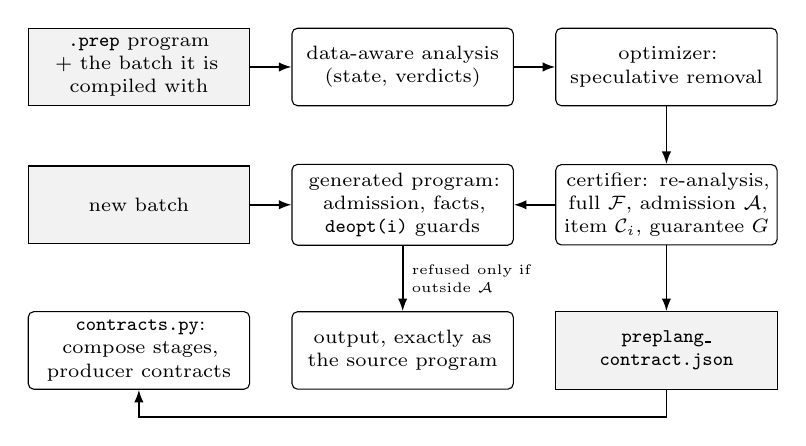
\begin{tikzpicture}[
    box/.style={draw, rounded corners=2pt, align=center, font={\fontsize{7}{8.4}\selectfont}, minimum height=2.8em,
                text width=2.6cm, inner sep=3pt},
    data/.style={draw, align=center, font={\fontsize{7}{8.4}\selectfont}, minimum height=2.8em, text width=2.6cm,
                 inner sep=3pt, fill=black!5},
    arr/.style={-{Latex[length=1.6mm]}, semithick},
    lbl/.style={font={\fontsize{5.5}{6.6}\selectfont}, align=left, inner sep=1pt}]
  \node[data] (src) at (0, 0) {\texttt{.prep} program\\+ the batch it is\\compiled with};
  \node[box] (ana) at (3.35, 0) {data-aware analysis\\(state, verdicts)};
  \node[box] (opt) at (6.7, 0) {optimizer:\\speculative removal};
  \node[box] (cer) at (6.7, -1.75) {certifier: re-analysis,\\full $\mathcal{F}$, admission $\mathcal{A}$,\\item $\mathcal{C}_i$, guarantee $G$};
  \node[box] (gen) at (3.35, -1.75) {generated program:\\admission, facts,\\\texttt{deopt(i)} guards};
  \node[data] (new) at (0, -1.75) {new batch};
  \node[box] (out) at (3.35, -3.6) {output, exactly as\\the source program};
  \node[data] (con) at (6.7, -3.6) {\texttt{preplang\_}\\\texttt{contract.json}};
  \node[box] (cmp) at (0, -3.6) {\texttt{contracts.py}:\\compose stages,\\producer contracts};
  \draw[arr] (src) -- (ana);
  \draw[arr] (ana) -- (opt);
  \draw[arr] (opt) -- (cer);
  \draw[arr] (cer) -- (gen);
  \draw[arr] (new) -- (gen);
  \draw[arr] (gen) -- node[lbl, right=2pt] {refused only if\\outside $\mathcal{A}$} (out);
  \draw[arr] (cer) -- (con);
  \draw[arr] (con.south) -- ++(0, -0.35) -| (cmp.south);
\end{tikzpicture}
\end{adjustbox}
\caption{How \PL compiles once and reuses the result. The certifier re-runs the analysis with weaker
input facts, reading no data; on a new batch, the generated program runs a removed instruction $i$
only if the batch breaks its item certificate $\mathcal{C}_i$.}
\label{fig:arch}
\end{figure}


The repository also holds \texttt{proofs/} (\LeanLines{} lines of Lean~4~\cite{lean4}). They prove two
things: for any sound and monotone analysis, the generated program gives the output of a fresh compilation
on every batch it admits; and the analysis of a core of the language is sound and monotone. Joins, groups,
dates and images are outside that core. Joins and groups are checked by the differential test of
Section~\ref{sec:impact}, dates and images only by unit tests and the examples. The other folders are \texttt{tests/} (\TestCount{} checks in \TestSuites{} suites), the pandas lifter
(\texttt{frontend/}), the tools below (\texttt{tools/}), a VS Code extension and the evaluation
(\texttt{eval/}).

\PL installs with \texttt{pip} from the repository (commands \texttt{preplang}, \texttt{preplang-lift},
\texttt{preplang-contracts}, \texttt{preplang-release-facts}) or runs from the \texttt{Dockerfile}.
Continuous integration builds and tests the compiler on Windows (MSVC), Ubuntu and macOS (GCC), compiles
every example, runs the tests under AddressSanitizer and UndefinedBehaviorSanitizer with a coverage gate,
fuzzes the three readers of untrusted bytes (\texttt{.prep}, CSV, Parquet footers) with libFuzzer, and
checks the Lean proofs. \texttt{LANGUAGE.md} documents the language, the
command line and the generated program; \texttt{ARCHITECTURE.md} maps each phase to its files.

\subsection{Software functionalities}

{\sloppy
\begin{itemize}
\item \textbf{Compile-time checking.} Misspelled or removed columns, type errors and broken contracts
(\texttt{NOT\_NULL}, \texttt{BETWEEN}, \texttt{UNIQUE}, \texttt{REFERENCES}, schemas, image channels and
sizes, match rates of images and labels) and lookup joins on keys of other types or with repeated values
are reported with the line, the offending row and a hint. Groups (\texttt{AGGREGATE}) keep their facts.
\item \textbf{Data-driven optimization.} Proven checks and operations without effect are removed, unused
columns are not loaded, and image pipelines are streamed. Rewrites that change the output, such as merging
two \texttt{RESIZE}s, are applied only with \texttt{--approx}.
\item \textbf{Tools around the compiler.} \texttt{tools/\allowbreak contracts.py} checks one compiled stage's
guarantees against the next stage's certificates; \texttt{frontend/\allowbreak pandas2prep.py} lifts the
cleaning part of pandas scripts into \PL, up to the first statement the language cannot express; and with
\texttt{--facts} a program compiles from differentially private facts that its data owner released
(\texttt{tools/\allowbreak release\_facts.py}) without opening an input file; the generated program checks
those facts on the real data, so every run stays exact.
\item \textbf{Inspection.} Every phase can be printed (\texttt{--tokens} to \texttt{--python}), together with
an execution plan (\texttt{--explain}), the files a run would touch (\texttt{--dry-run}) and the
diagnostics as JSON (\texttt{--json}).
\end{itemize}
}

\section{Illustrative example}\label{sec:example}

\begin{lstlisting}
LOAD "students.csv" AS students;
EXPECT students.age NUMBER;
EXPECT students.marks BETWEEN 0 AND 100;
EXPECT students.name NOT_NULL;
FILTER students WHERE marks >= 50;
EXPECT students.marks BETWEEN 60 AND 100;
SAVE students AS "clean.csv";
\end{lstlisting}

Compiled against an eight-row \texttt{students.csv} (from \texttt{examples/\allowbreak tabular/}),
\PL proves the first three contracts. It keeps the fourth as a run-time check, since after the filter it
knows only that the marks lie in $[50, 95]$. It removes the range and not-null checks speculatively, and
\texttt{--certificate} shows the facts the range check needs: marks at least 0 and at most 100. Run on a
later batch in which a mark is 104, the generated program re-enables the check and stops where a fresh
compilation would:
{\small\begin{verbatim}
Deoptimized line 3: EXPECT students.marks BETWEEN 0 AND 100:
  marks goes up to 104, above 100
ContractError: line 3: students.marks has values outside 0 to 100
\end{verbatim}}
\noindent A batch within the facts runs with both checks removed. A batch whose \texttt{age} holds text is
refused, because generated code cannot replace an analysis of the column under another type.

The same analysis covers images, from their headers alone. In \texttt{examples/\allowbreak images/\allowbreak
linked.prep}, images and their labels are linked and checked, resized, normalized to $[0, 1]$ and saved as
NumPy arrays. Changing the format to PNG gives, before any pixel is decoded:
{\small\begin{verbatim}
error[type]: cannot save FLOAT32 pixels as PNG:
             NORMALIZE at line 10 scaled them to [0, 1]
   --> examples/images/linked.prep:13:1
13 | SAVE_IMAGES imgs TO "processed/ml_ready/";
   = hint: image files store 8-bit pixels, so these would come out
     almost black; add CONVERT imgs TO NPY; to keep the float
     values
\end{verbatim}}
\noindent The equivalent hand-written OpenCV script runs without an error and writes almost black images.

\section{Impact}\label{sec:impact}

\PL is a research prototype by one author, begun in a compiler-design course, and has no users outside
the author's experiments yet. Its evidence is the evaluation in \texttt{eval/}; \texttt{eval/\allowbreak
evaluate.py} writes every number below from the raw results.

\begin{itemize}
\item \textbf{Correctness.} \DiffPrograms{} random programs (with joins and groups), compiled with and
without the optimizer, agree cell by cell with a reference interpreter written in Python that shares no
code with the compiler. Reused on a second random batch, none of \DiffReuse{} runs differs from it. This
test found two bugs (column pruning, a pandas~3 incompatibility) that had made \DiffBeforeWrongOpt{}
optimized runs wrong, and three more seeds (\DiffSeedPrograms{} programs) found a third (a statistic fill
removed as a dead store, \DiffSeedBeforeWrong{} wrong run); after the fixes all \DiffSeedAgree{} agree
and none of \DiffSeedReuse{} reuses is wrong. The CSV fuzzer found an out-of-bounds read on a NUL byte.
Each fix has a regression test.
\item \textbf{Performance.} On a table of 200{,}000 rows the optimized program runs in \TabProcOpt\,s
instead of \TabProcOz\,s after Python start-up. An image pipeline runs as fast as a hand-written
streaming script, in \ImgPlMem\,MiB instead of the \ImgBaseMem\,MiB of a script that loads every image.
\item \textbf{Optimization.} On \CenPrograms{} programs (the examples and programs lifted from GitHub
scripts) the optimizer removes \CenInstrCut\% of the instructions (\CenInstrBefore{} to \CenInstrAfter),
\CenChecksBefore{} to \CenChecksAfter{} run-time checks and \CenColsCut\% of the columns read, and changes
\CenChanged{} programs; all \CenSame{} write the same files with and without it. The lifted scripts
contain no contracts, so all removed checks come from the examples and the three monthly pipelines.
\item \textbf{Real programs.} Of \RbTotal{} data-preparation failures reported in GitHub issues, \RbEarly{}
are reported before any data is processed (\RbContract{} of them only after the requirement is written as an
\texttt{EXPECT}). Of \CorpusBothScripts{} Titanic and House Prices scripts from GitHub the lifter
translates \CorpusBothLifted{}; their programs reproduce a fresh compilation in \CorpusBothSame{} of
\CorpusBothRuns{} runs on new batches, refuse the other 14, and are never wrong. Of \DriftAll{} traffic and
bike scripts it translates \DriftCompiled{}, which reproduce a fresh run on all \DriftRuns{} later real
months. Most untranslated scripts fail before the language matters: 547 of the 945 never call
\texttt{pd.read\_csv} on a file path, which the lifter needs to find the input.
\item \textbf{Comparison.} Three monthly pipelines, compiled once and run on \RealRuns{} later real months
(UCI traffic and bikes, NYC taxi), handle \RealDeoptCorrect{} (\RealDeoptCorrectPct\%) as a fresh
compilation would and none wrongly; the \RealDeoptNeedless{} they refuse are taxi months in which
\texttt{passenger\_count} changed type. The validators answer the same question, whether the pipeline may
run on a month: each learns from the month the pipeline was compiled on, as its documentation suggests
(Great Expectations profiles the columns, pandera and TFDV infer a schema), and every answer is scored against a fresh
compilation of the month. Great Expectations and pandera refuse
\RealValidatorStopMin--\RealValidatorStopMax\% of the months, and TFDV admits \RealValidatorWrongMax{}
months on which the program then differs. The validators were not built for this decision; the numbers
show what it costs to use them for it. All 24 mistakes injected into 5 example programs are reported at
compile time, where a script-style pandas program crashes on 20 and writes wrong output on 4.
\item \textbf{Private compilation.} At $\varepsilon=1$ the private facts keep every removal of the taxi
and traffic pipelines but only 14\% of the bikes pipeline's, where AIM~\cite{mckenna2022aim} with its
own workload keeps 54\%. On the \PrivTitanicScripts{} Titanic scripts, \PrivTitanicDeoptEpsOne{}
compilations remove instructions that their own input then re-enables, because a released fact was
false. In all \PrivRuns{} runs after \PrivCompilations{} private compilations no output differs
from a fresh compilation.
\item \textbf{Overhead.} Compiling takes a median of \CenCompileMed\,ms and at most \CenMemMax\,MiB
(\CenCsvMillionMem\,MiB for a million CSV rows). Checking the certificate of a new batch changes run time
by \OhPctLow\% to \OhPctHigh\%, within measurement noise.
\end{itemize}

\noindent \texttt{eval/\allowbreak reproduce.sh check} (about ten minutes, no network) rebuilds the compiler,
runs every test, regenerates every number above from the committed results, and reruns small versions of
the differential test and the optimization census, which the Docker image can also run.
\texttt{full} (several hours) downloads the inputs and reruns every experiment, and \texttt{baselines}
reruns the validators, in pinned environments. The GitHub script corpora are frozen as evaluated, each
file by its URL at a fixed commit and its hash.

\section{Limitations and conclusions}

Joins are lookups on a key with one name in both tables (no many-to-many joins), groups have five
aggregates, and only Python is generated. A changed column type is refused rather than handled. The
mechanized proofs do not cover joins, groups, dates or images. The lifter translated a minority of the
GitHub scripts above. The comparison with validators uses three pipelines written by the author, and
\PL has no outside users yet and no user study; \texttt{docs/\allowbreak USER\_STUDY.md} is its protocol. Planned work is general joins,
generated code that adapts to type changes, and that study, with people who write pandas cleaning scripts.


\section*{CRediT authorship contribution statement}
\textbf{Nikhil V:} Conceptualization, Methodology, Software, Validation, Investigation, Data curation,
Visualization, Writing -- original draft. \textbf{Ranjithkumar S:} Supervision, Writing -- review and
editing.

\section*{Declaration of competing interest}
The authors declare that they have no known competing financial interests or personal relationships that
could have appeared to influence the work reported in this paper.

\section*{Funding}
This research did not receive any specific grant from funding agencies in the public, commercial, or
not-for-profit sectors.

\section*{Data availability}
The source code, the evaluation scripts and every raw result are in the repository of the metadata table
(C2), under the MIT license. The public datasets are downloaded by \texttt{eval/\allowbreak reproduce.sh};
the GitHub script corpora are pinned there by URL, commit and hash.

% Science of Computer Programming requires this statement, before the references, when generative AI
% tools were used; the section title is the one the Guide for Authors gives.
\section*{Declaration of generative AI and AI-assisted technologies in the manuscript preparation process}
Generative AI tools assisted with implementation, literature search, evaluation scripts, analysis and
drafting of this manuscript. The authors reviewed all text, code and results and take responsibility
for them.

% Written by osp_references.py from sections/references.tex; do not edit by hand.
\begin{thebibliography}{99}
\footnotesize
\bibitem{sculley2015}
D. Sculley, G. Holt, D. Golovin, E. Davydov, T. Phillips, D. Ebner, V. Chaudhary, M. Young, J.-F.
Crespo, and D. Dennison, ``Hidden technical debt in machine learning systems,'' in \emph{Advances
in Neural Information Processing Systems (NeurIPS)}, 2015, pp. 2503--2511.

\bibitem{mckinney2010}
W. McKinney, ``Data structures for statistical computing in Python,'' in \emph{Proc. 9th Python in
Science Conf. (SciPy)}, 2010, pp. 56--61. \url{https://doi.org/10.25080/Majora-92bf1922-00a}.

\bibitem{bradski2000}
G. Bradski, ``The OpenCV library,'' \emph{Dr. Dobb's Journal of Software Tools}, 2000.

\bibitem{breck2019}
E. Breck, N. Polyzotis, S. Roy, S. E. Whang, and M. Zinkevich, ``Data validation for machine
learning,'' in \emph{Proc. Conf. on Machine Learning and Systems (MLSys)}, 2019.

\bibitem{schelter2018}
S. Schelter, D. Lange, P. Schmidt, M. Celikel, F. Biessmann, and A. Grafberger, ``Automating
large-scale data quality verification,'' \emph{Proc. VLDB Endowment}, vol. 11, no. 12,
pp. 1781--1794, 2018. \url{https://doi.org/10.14778/3229863.3229867}.

\bibitem{gx}
Great Expectations, ``Great Expectations: data quality testing,'' \url{https://greatexpectations.io}.

\bibitem{bantilan2020}
N. Bantilan, ``pandera: Statistical data validation of pandas dataframes,'' in \emph{Proc. 19th
Python in Science Conf. (SciPy)}, 2020, pp. 116--124. \url{https://doi.org/10.25080/Majora-342d178e-021}.

\bibitem{preplang2026}
Nikhil V, PrepLang, version 2.1.0 [Computer software], GitHub, 2026.
\url{https://github.com/Nikhi00718/preLang/tree/v2.1.0}.

\bibitem{petricek2016}
T. Petricek, G. Guerra, and D. Syme, ``Types from data: Making structured data first-class citizens
in F\#,'' in \emph{Proc. 37th ACM SIGPLAN Conf. on Programming Language Design and Implementation
(PLDI)}, 2016, pp. 477--490. \url{https://doi.org/10.1145/2908080.2908115}.

\bibitem{godfrey2001}
P. Godfrey, J. Gryz, and C. Zuzarte, ``Exploiting constraint-like data characterizations in query
optimization,'' in \emph{Proc. ACM SIGMOD Int. Conf. on Management of Data}, 2001, pp. 582--592.
\url{https://doi.org/10.1145/375663.375749}.

\bibitem{holzle1992}
U. H\"olzle, C. Chambers, and D. Ungar, ``Debugging optimized code with dynamic deoptimization,'' in
\emph{Proc. ACM SIGPLAN Conf. on Programming Language Design and Implementation (PLDI)}, 1992,
pp. 32--43. \url{https://doi.org/10.1145/143103.143114}.

\bibitem{barriere2021}
A. Barrière, S. Blazy, O. Flückiger, D. Pichardie, and J. Vitek, ``Formally verified speculation and
deoptimization in a JIT compiler,'' \emph{Proc. ACM Program. Lang.}, vol. 5, no. POPL, pp. 1--26, 2021. \url{https://doi.org/10.1145/3434327}.

\bibitem{spiegelberg2021}
L. Spiegelberg, R. Yesantharao, M. Schwarzkopf, and T. Kraska, ``Tuplex: Data science in Python at
native code speed,'' in \emph{Proc. ACM SIGMOD Int. Conf. on Management of Data}, 2021,
pp. 1718--1731. \url{https://doi.org/10.1145/3448016.3457244}.

\bibitem{schelter2024screening}
S. Schelter, S. Guha, and S. Grafberger, ``Automated provenance-based screening of ML data preparation
pipelines,'' \emph{Datenbank-Spektrum}, vol. 24, no. 3, pp. 187--196, 2024.
\url{https://doi.org/10.1007/s13222-024-00483-4}.

\bibitem{zhuang2022}
Y. Y. Zhuang and M.-Y. Lu, ``Enabling type checking on columns in data frame libraries by abstract
interpretation,'' \emph{IEEE Access}, vol. 10, 2022. \url{https://doi.org/10.1109/ACCESS.2022.3146287}.

\bibitem{gerstl2026}
O. Gerstl, F. Sihler, and M. Tichy, ``Inferring the shape of data frames in R programs using
abstract interpretation,'' arXiv preprint arXiv:2607.03889, 2026.
\url{https://doi.org/10.48550/arXiv.2607.03889}.

\bibitem{mirji2026}
V. Mirji, ``Shift schema drift left: Policy-aware compile-time contracts for typed JVM and Spark
pipelines,'' arXiv preprint arXiv:2604.16986, 2026.
\url{https://doi.org/10.48550/arXiv.2604.16986}.

\bibitem{lean4}
L. de Moura and S. Ullrich, ``The Lean 4 theorem prover and programming language,'' in \emph{Proc.
28th Int. Conf. on Automated Deduction (CADE)}, LNCS 12699, 2021, pp. 625--635.
\url{https://doi.org/10.1007/978-3-030-79876-5_37}.

\bibitem{mckenna2022aim}
R. McKenna, B. Mullins, D. Sheldon, and G. Miklau, ``AIM: An adaptive and iterative mechanism for
differentially private synthetic data,'' \emph{Proc. VLDB Endowment}, vol. 15, no. 11, pp. 2599--2612,
2022. \url{https://doi.org/10.14778/3551793.3551817}.

\end{thebibliography}


\end{document}
